\documentclass[11pt,a4paper]{ctexart}

\usepackage[margin=2.4cm]{geometry}
\usepackage{amsmath,amssymb,mathtools,empheq}
\usepackage{booktabs,array,multirow}
\usepackage{graphicx}
\usepackage{xcolor}
\usepackage{listings}
\usepackage{caption}
\usepackage{enumitem}
\usepackage{fancyhdr}
\usepackage[colorlinks,linkcolor=blue!50!black,urlcolor=blue!50!black]{hyperref}

\definecolor{codebg}{RGB}{248,249,251}
\definecolor{codekw}{RGB}{0,90,160}
\definecolor{codecm}{RGB}{110,120,130}
\definecolor{codestr}{RGB}{160,70,20}

\lstdefinestyle{py}{
  language=Python, backgroundcolor=\color{codebg}, basicstyle=\ttfamily\small,
  keywordstyle=\color{codekw}\bfseries, commentstyle=\color{codecm}\itshape,
  stringstyle=\color{codestr}, numbers=left, numberstyle=\tiny\color{gray},
  frame=single, rulecolor=\color{gray!40}, breaklines=true, showstringspaces=false,
  xleftmargin=1.6em, framexleftmargin=1.4em, aboveskip=1em, belowskip=1em
}
\lstset{style=py}

\newcommand{\keypoint}[1]{\par\medskip\noindent\colorbox{cyan!6}{%
  \begin{minipage}{\dimexpr\linewidth-2\fboxsep}\small #1\end{minipage}}\par\medskip}

\pagestyle{fancy}
\fancyhf{}
\lhead{\small Transformer 从零实现}
\rhead{\small\thepage}
\renewcommand{\headrulewidth}{0.4pt}

\title{\textbf{Transformer 从零实现}\\[4pt]
\large 背景 · 推导 · 前向反向 · 纯 numpy 与 torch 双实现 · 可视化}
\author{倒立摆控制课程 · 第二部}
\date{}

\begin{document}
\maketitle

\begin{abstract}
\noindent
这份教程只做一件事：把一个小型因果 Transformer（18,177 个参数）从\textbf{动机}写到
\textbf{可以逐行读懂的实现}，并保证读者能自己验证它是对的。具体地——

\begin{itemize}[leftmargin=1.4em,itemsep=2pt]
  \item 解释它为什么长这样：RNN 的两个硬伤、注意力的"检索"解释；
  \item 给出每一层的前向公式与\textbf{反向雅可比}（softmax、LayerNorm、GELU、残差）；
  \item 提供\textbf{纯 numpy 手写反向}与 \textbf{torch autograd} 两份实现，
        二者的前向输出差 $3\times10^{-15}$、全部 31 个参数张量的梯度差 $3\times10^{-14}$；
  \item 用中心差分做与框架无关的第三方验证；
  \item 给出训练曲线、一致性散点、注意力热图三张可视化。
\end{itemize}

\noindent
所有代码在 \texttt{tutorial/code/}，所有数字都可以用 \texttt{parity\_test.py} 与
\texttt{train\_demo.py} 复现。
\end{abstract}

\tableofcontents
\newpage

\section{背景：为什么需要 Transformer}

\subsection{序列建模的三代方案}

我们要学的是一个映射 $\pi:\ \mathbb{R}^{T\times F}\to\mathbb{R}$（$T$ 步历史、每步 $F$ 维特征，
输出一个标量）。历史上解决它有三条路：

\begin{center}
\small
\begin{tabular}{@{}llll@{}}
\toprule
方案 & 关键运算 & 参数随 $T$ 增长 & 任意两步的"路径长度" \\
\midrule
MLP（展平） & $W\,\mathrm{vec}(x)$ & 线性增长 & $1$（但无结构先验）\\
RNN & $h_t=f(h_{t-1},x_t)$ & 不增长 & $O(|t-s|)$ 步 \\
Attention & $\sum_s a_{ts}v_s$ & 不增长 & $O(1)$ \\
\bottomrule
\end{tabular}
\end{center}

\subsection{RNN 的两个硬伤}

设 $h_t=\tanh(Wh_{t-1}+Ux_t)$。沿时间反传时，梯度要连乘
\begin{equation}
  \frac{\partial h_t}{\partial h_s}=\prod_{k=s+1}^{t}\frac{\partial h_k}{\partial h_{k-1}}
  =\prod_{k}\mathrm{diag}\big(1-\tanh^2(\cdot)\big)W .
\end{equation}
若 $W$ 的最大奇异值 $\sigma<1$，连乘\textbf{指数衰减}（梯度消失）；$\sigma>1$ 则指数爆炸。
这是第一个硬伤：\textbf{长程依赖无法稳定学习}。

第二个硬伤是工程性的：$h_t$ 依赖 $h_{t-1}$，\textbf{无法并行}。一条 $T=1000$ 的序列，
训练时只能串行展开 $1000$ 次。

\begin{quote}
\textbf{Transformer 的两个回答}：
（1）让任意两个位置\textbf{直接相连}（路径长度 $O(1)$）；
（2）让所有位置\textbf{同时计算}（矩阵乘法的并行性）。
\end{quote}

\subsection{检索视角：注意力到底是什么}

把历史看成一张"键值表" $\{(k_s,v_s)\}_{s\le t}$，当前时刻有一个"查询" $q_t$。
我们要的是"\textbf{按需回看}"：找到与 $q_t$ 最相关的 $k_s$，取出对应的 $v_s$。

硬检索是 $\arg\max_s q_t^\top k_s$——不可微，无法训练。把它软化：
\begin{equation}
  a_{ts}=\frac{\exp(q_t^\top k_s/\sqrt{d_h})}{\sum_{s'\le t}\exp(q_t^\top k_{s'}/\sqrt{d_h})},
  \qquad
  y_t=\sum_{s\le t}a_{ts}\,v_s .
  \label{eq:attn}
\end{equation}
$a_{ts}$ 就是\textbf{注意力权重}，$y_t$ 是值的加权平均。整个式 \eqref{eq:attn} 对
$q,k,v$ 都是可微的，于是可以用梯度下降学习"该看哪里"。

\section{结构总览}

\subsection{数据流与张量形状}

\begin{center}
\small
\begin{tabular}{@{}clcl@{}}
\toprule
步 & 运算 & 形状 & 参数量 \\
\midrule
1 & 输入窗口 $x$ & $B\times T\times F$ & -- \\
2 & 线性嵌入 $W_{\text{in}}x+b$ & $B\times T\times d$ & $dF+d$ \\
3 & 加可学习位置编码 & $B\times T\times d$ & $Td$ \\
4 & LN1 & $B\times T\times d$ & $2d$ \\
5 & QKV 投影 & $B\times T\times 3d$ & $3d^2+3d$ \\
6 & 分头 $\to$ 缩放点积 + 因果掩码 & $B\times H\times T\times T$ & -- \\
7 & softmax $\to$ 加权求和 $AV$ & $B\times H\times T\times d_h$ & -- \\
8 & 合并 + 输出投影 & $B\times T\times d$ & $d^2+d$ \\
9 & 残差 $z\leftarrow z+\cdot$ & $B\times T\times d$ & -- \\
10 & LN2 $\to$ FFN($d\to f\to d$) & $B\times T\times d$ & $2df+f+d$ \\
11 & 残差 & $B\times T\times d$ & -- \\
12 & $4$--$11$ 重复 $L$ 次 & & \\
13 & 取最后 token $\to$ LN $\to$ 线性 & $B\times 1$ & $2d+d+1$ \\
14 & $u=u_{\max}\tanh(\cdot)$ & $B$ & -- \\
\bottomrule
\end{tabular}
\end{center}

本教程取 $T=24,\ F=6,\ d=32,\ H=4,\ d_h=8,\ f=64,\ L=2$，合计
\begin{equation}
  \underbrace{(6\cdot32+32)}_{224}+\underbrace{24\cdot32}_{768}
  +2\cdot\underbrace{(2\cdot32+3\cdot32^2+3\cdot32+32^2+32+2\cdot32+64\cdot32+64+32\cdot64+32)}_{8544}
  +2\cdot32+33=\mathbf{18{,}177}.
\end{equation}

\subsection{一个必须强调的约束：因果性}

解码器式的模型只能看过去。实现上在 softmax 之前把上三角位置置 $-\infty$：
\begin{equation}
  M_{ts}=\begin{cases}0,& s\le t\\-\infty,& s>t\end{cases},\qquad
  s_{ts}=\frac{q_t^\top k_s}{\sqrt{d_h}}+M_{ts}.
\end{equation}
\begin{quote}
\textbf{训练时也必须加掩码}。否则模型会学到一个依赖未来输入的"作弊解"：
训练损失极低，部署时那些输入根本不存在。这是实现中最容易犯且最难发现的错误之一。
\end{quote}

\section{逐层前向与反向}

\subsection{LayerNorm}

前向（对最后一维归一化）：
\begin{equation}
  \mu=\frac1d\sum_i z_i,\quad \sigma^2=\frac1d\sum_i(z_i-\mu)^2,\quad
  \hat z=\frac{z-\mu}{\sqrt{\sigma^2+\varepsilon}},\quad y=\hat z\odot\gamma+\beta .
\end{equation}
反向的紧凑形式（$\bar g$ 表示对最后一维取均值）：
\begin{equation}
  \frac{\partial\mathcal{L}}{\partial z}
  =\frac{\gamma}{\sigma}\Big(g-\bar g-\hat z\,\overline{(g\odot\hat z)}\Big),
  \qquad g=\frac{\partial\mathcal{L}}{\partial y}.
  \label{eq:lnback}
\end{equation}

\begin{quote}
括号里两项分别在\textbf{抵消整体平移}与\textbf{整体缩放}方向的梯度分量。
这解释了两件事：（1）LN 让每层输入的尺度一致，是 Pre-LN 结构稳定的根源；
（2）它的梯度天然正交于两个"无用方向"，不会把残差主干推歪。
\end{quote}

\subsection{多头因果注意力}

前向（单头，$d_h=d/H$）：
\begin{align}
  q&=hW_q^\top,\quad k=hW_k^\top,\quad v=hW_v^\top,\\
  s&=\frac{qk^\top}{\sqrt{d_h}}+M,\qquad a=\mathrm{softmax}(s),\\
  y&=a\,v .
\end{align}

\textbf{为什么除以 $\sqrt{d_h}$}：设 $q_i,k_i$ 独立、零均值、单位方差，则
\begin{equation}
  q^\top k=\sum_{i=1}^{d_h}q_ik_i\ \Rightarrow\
  \mathbb{E}[q^\top k]=0,\quad \mathrm{Var}(q^\top k)=d_h .
\end{equation}
点积的标准差是 $\sqrt{d_h}$；不缩放会让 softmax 的输入分布过宽而饱和（梯度趋近 $0$）。
本教程 $d_h=8$，缩放因子 $\sqrt8\approx2.83$。

\textbf{反向}。记 $Y=AV$，$S$ 为 softmax 之前的分数，$G=\partial\mathcal{L}/\partial Y$：
\begin{align}
  \frac{\partial\mathcal{L}}{\partial A}&=G\,V^\top, &
  \frac{\partial\mathcal{L}}{\partial V}&=A^\top G,\\
  \frac{\partial\mathcal{L}}{\partial S}&=A\odot\Big(\frac{\partial\mathcal{L}}{\partial A}
   -\sum_j A_{j}\,\frac{\partial\mathcal{L}}{\partial A_{j}}\Big), &
  \frac{\partial\mathcal{L}}{\partial Q}&=\frac{1}{\sqrt{d_h}}\frac{\partial\mathcal{L}}{\partial S}K,\quad
  \frac{\partial\mathcal{L}}{\partial K}=\frac{1}{\sqrt{d_h}}\Big(\frac{\partial\mathcal{L}}{\partial S}\Big)^\top Q .
\end{align}

\begin{quote}
\textbf{softmax 的雅可比自带"减基线"}：$\partial a_i/\partial s_j=a_i(\delta_{ij}-a_j)$，
链式展开后就出现 $-\sum_j a_j g_j$ 这一项。它的作用是\textbf{把梯度的均值减掉}——
若所有 $g_j$ 相同，梯度为零（因为此时改变分数不改变 softmax 输出）。
\keypoint{实现提示：掩码位置 $a_{ts}=0$，因此由上式得到的 $\partial\mathcal{L}/\partial S$ 在那里
\textbf{自动为零}，不需要额外写 masked\_fill。}
\end{quote}

\subsection{GELU}

\begin{equation}
  \mathrm{GELU}(x)=\tfrac12x\big(1+\mathrm{erf}(x/\sqrt2)\big),\qquad
  \frac{d}{dx}\mathrm{GELU}(x)=\tfrac12\big(1+\mathrm{erf}(x/\sqrt2)\big)
  +\frac{x}{\sqrt{2\pi}}e^{-x^2/2}.
\end{equation}
与 ReLU 的区别：负半轴不是硬截断而是\textbf{软门控}，实测 $64$ 个隐单元中有 $34$ 个输入为负，
它们被压到 $[-0.17,0)$ 而不是 $0$。

\subsection{残差与输出头}

残差把前向写成 $z\leftarrow z+f(z)$，反向时
\begin{equation}
  \frac{\partial\mathcal{L}}{\partial z}=\frac{\partial\mathcal{L}}{\partial z_{\text{out}}}
  \Big(I+\frac{\partial f}{\partial z}\Big),
\end{equation}
单位阵 $I$ 就是"梯度高速公路"：即使 $\partial f/\partial z$ 很小，梯度也能原样传回去。

输出层 $u=u_{\max}\tanh(r)$：
\begin{equation}
  \frac{\partial u}{\partial r}=u_{\max}\big(1-\tanh^2r\big).
\end{equation}
$|u|$ 接近 $u_{\max}$ 时导数趋于 $0$（饱和），这是"用 $\tanh$ 限幅"的代价。

\section{纯 numpy 实现}

\subsection{代码骨架}

\begin{lstlisting}[caption={tinytf\_numpy.py 的核心结构}]
class TinyTF:
    def forward(self, x, return_cache=False):
        z = x @ self.p["W_in"].T + self.p["b_in"] + self.p["pos"]   # (B,T,d)
        for l in range(self.L):
            h, c_ln1 = ln_forward(z, g1, b1)          # LN1
            q, k, v = self.qkv(h)                     # (B,H,T,dh)
            a = softmax(mask(q @ k.transpose / sqrt(dh)))
            z = z + self.proj(merge(a @ v))           # 残差 1
            h2, c_ln2 = ln_forward(z, g2, b2)         # LN2
            z = z + self.fc2(gelu(self.fc1(h2)))      # 残差 2
            cache.append(...)                         # 存所有中间量
        r = self.head(ln(z[:, -1]))                   # 只取最后一个 token
        return self.u_max * np.tanh(r)

    def backward(self, dU, cache):
        # 反向走一遍：tanh -> head -> LN -> 每层(FFN -> LN2 -> 残差 -> 注意力 -> LN1 -> 残差)
        ...
\end{lstlisting}

\subsection{五个易错点}

这一节是本教程的"避坑清单"——每一条我都在实现中真实踩过。

\begin{enumerate}[leftmargin=1.6em,itemsep=4pt]
  \item \textbf{多头 reshape 的顺序}。$(B,T,d)\to(B,T,H,d_h)$ 之后必须
        \texttt{transpose(1,2)} 变成 $(B,H,T,d_h)$，否则"头"会切在时间维上。
        反传时要逆序做 \texttt{transpose(0,2,1,3).reshape(B,T,d)}。
  \item \textbf{softmax 的减基线项不能漏}。只写 $A\odot\frac{\partial\mathcal{L}}{\partial A}$
        会漏掉 $-\sum_jA_jg_j$，梯度整体偏移，训练仍能下降但收敛变差。
  \item \textbf{LayerNorm 用紧凑式}。按 $d\mu,d\sigma^2$ 逐步展开也能推出来，
        但式 \eqref{eq:lnback} 更短且数值更稳。
  \item \textbf{$W_2$ 与 $b_2$ 的梯度来自残差主干}。$z=z_1+W_2\,\mathrm{GELU}(W_1h_2)$：
        应该用 $\partial\mathcal{L}/\partial z$（主干）而不是 $\partial\mathcal{L}/\partial \mathrm{act}$
        ——我最初写成了后者，形状立刻从 $(d,f)$ 变 $(f,f)$，被形状检查抓到。
  \item \textbf{掩码位置的梯度}。不需要显式清零：$a=0\Rightarrow \partial\mathcal{L}/\partial S=0$。
        但如果用 $-1e4$ 而不是 $-\infty$，$a$ 会是 $10^{-4343}\approx0$（仍是 $0$），安全；
        用 $-1$ 就错了。
\end{enumerate}

\subsection{与 autograd 逐位对齐}

\texttt{parity\_test.py} 把同一套权重分别装进 numpy 版与 torch 版，
同一个损失函数、同一个上游梯度：

\begin{center}
\small
\begin{tabular}{@{}lcc@{}}
\toprule
量 & 最大绝对偏差 & 说明 \\
\midrule
前向输出 $u$ & $3.1\times10^{-15}$ & float64 舍入量级 \\
损失 $\mathcal{L}$ & $<10^{-15}$ & 完全一致 \\
31 个参数张量的梯度 & $\mathbf{3.0\times10^{-14}}$ & 手推反向 $\equiv$ autograd \\
\midrule
中心差分（$h=10^{-6}$，3 个抽样元素） & 相对误差 $5\times10^{-11}\sim8\times10^{-9}$ & 与框架无关的第三方证据 \\
\bottomrule
\end{tabular}
\end{center}

\begin{quote}
\textbf{这三行数字就是"实现正确"的定义}。
如果手推梯度有任何一个符号或转置错，偏差不会停在 $10^{-14}$，而会到 $10^{-2}$ 甚至形状不匹配。
\end{quote}

\section{torch 实现与训练对比}

\subsection{等价结构}

\begin{lstlisting}[caption={tinytf\_torch.py 的核心（与 numpy 版一一对应）}]
class Block(nn.Module):
    def forward(self, z, mask):
        B, T, d = z.shape
        q, k, v = self.qkv(self.ln1(z)).chunk(3, dim=-1)
        q, k, v = [t.view(B, T, self.h, self.nh).transpose(1, 2) for t in (q, k, v)]
        s = (q @ k.transpose(-1, -2)) / math.sqrt(self.nh)
        a = torch.softmax(s.masked_fill(mask, -1e9), dim=-1)
        z = z + self.proj((a @ v).transpose(1, 2).reshape(B, T, d))
        return z + self.fc2(F.gelu(self.fc1(self.ln2(z))))
\end{lstlisting}

两版共享权重布局：\texttt{state\_from\_numpy()} 把 numpy 的字典映射成 \texttt{state\_dict}，
反向映射是 \texttt{numpy\_from\_state()}。这让我们可以做三件事：
验证梯度、以 numpy 做推理、以及把生产权重装进 numpy 做可视化。

\subsection{训练对比}

同初始化、同数据（52,164 个训练窗口）、同批次顺序、同学习率调度，各训 8 个 epoch：

\begin{center}
\small
\begin{tabular}{@{}lccc@{}}
\toprule
 & 训练损失（8 epoch 末） & 验证损失 & 耗时 \\
\midrule
numpy（手写反向） & $3.60\times10^{-3}$ & $3.694\times10^{-3}$ & $142$\,s \\
torch（autograd） & $3.60\times10^{-3}$ & $3.695\times10^{-3}$ & $35$\,s \\
\midrule
差异 & $1.7\times10^{-7}$ & $1.3\times10^{-7}$ & 加速 $4.1\times$ \\
\bottomrule
\end{tabular}
\end{center}

\begin{figure}[htbp]
\centering
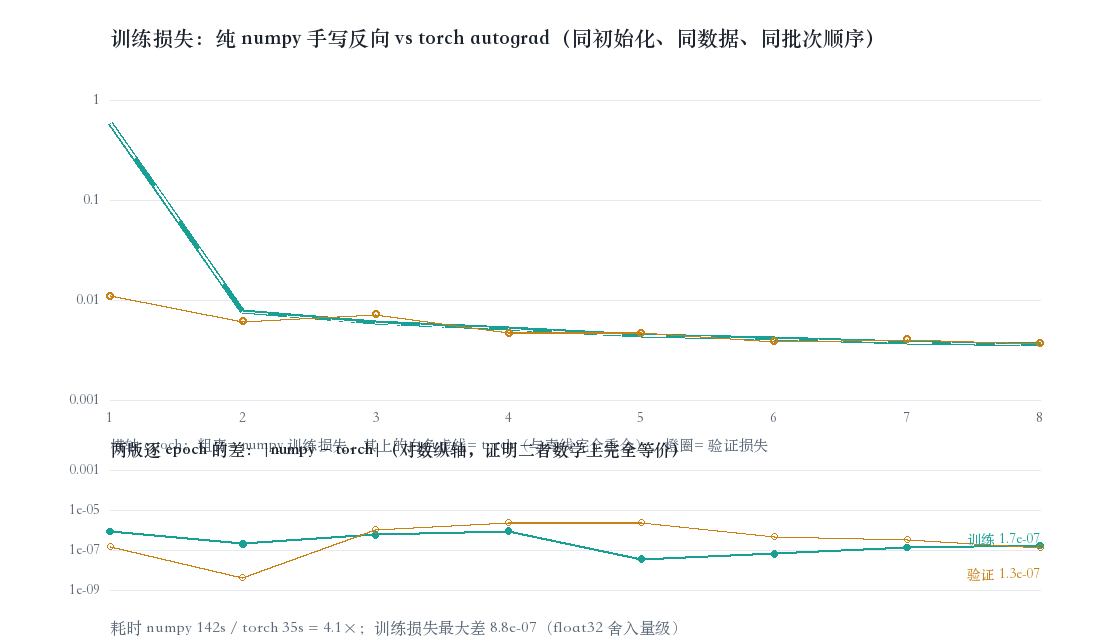
\includegraphics[width=0.96\linewidth]{../out/fig_loss.png}
\caption{上：训练/验证损失；粗青线是 numpy，其上白色虚线是 torch（两者完全重合）。
下：两版逐 epoch 的绝对差，稳定在 float32 舍入量级 $10^{-7}$。}
\end{figure}

\section{结果可视化}

\subsection{加载生产权重：一致性散点}

把本项目训练好的权重（BC+DAgger，闭环 $100\%$）装进 numpy 版，在 $512$ 个真实窗口上比较：

\begin{center}
\small
\begin{tabular}{@{}lcc@{}}
\toprule
指标 & 数值 & 说明 \\
\midrule
$\max|u_{\text{numpy}}-u_{\text{torch}}|$ & $5.4\times10^{-6}$\,N & float32 权重下 \\
平均偏差 & $8.1\times10^{-7}$\,N & $u_{\max}$ 的 $0.0000067\%$ \\
相关系数 & $1.000000000$ & -- \\
\midrule
闭环成功率（numpy 策略，30 组初值） & $30/30$ & 与 torch 版完全一致 \\
从下垂出发摆起用时 & $1.9$\,s & -- \\
\bottomrule
\end{tabular}
\end{center}

\begin{figure}[htbp]
\centering
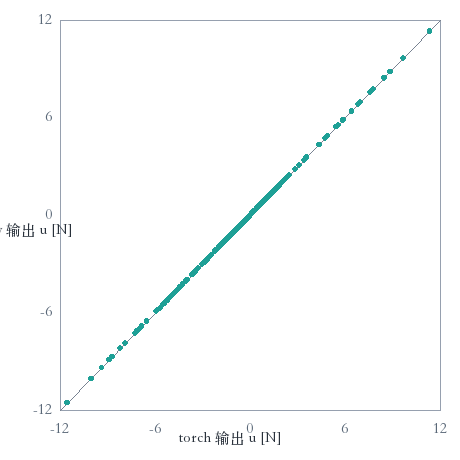
\includegraphics[width=0.42\linewidth]{../out/fig_parity.png}
\caption{numpy 与 torch 在同一批真实窗口上的输出。所有点落在 $y=x$ 上。}
\end{figure}

\subsection{注意力热图}

\begin{figure}[htbp]
\centering
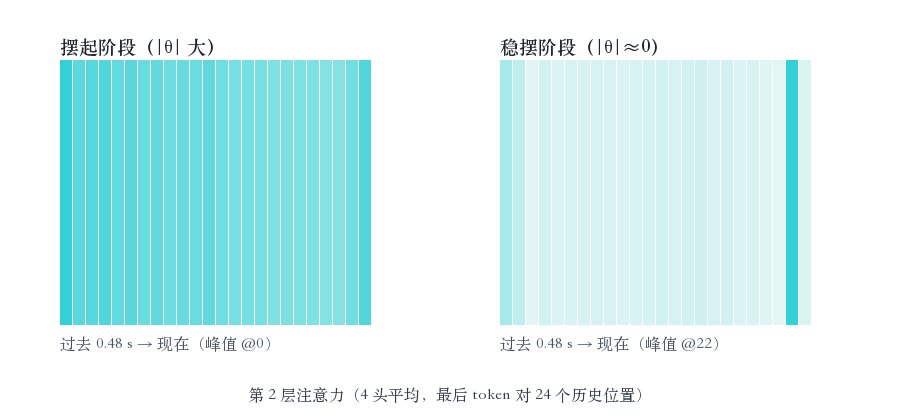
\includegraphics[width=0.96\linewidth]{../out/fig_attention.png}
\caption{第 2 层注意力（4 头平均，最后 token 对 24 个历史位置）。
左：摆起阶段，权重铺满整段（峰值偏早）；右：稳摆阶段，峰值锁在最近第 2 步。
这是"估相位"与"估变化率"两种信息需求的直接体现。}
\end{figure}

\subsection{梯度量级}

\begin{figure}[htbp]
\centering
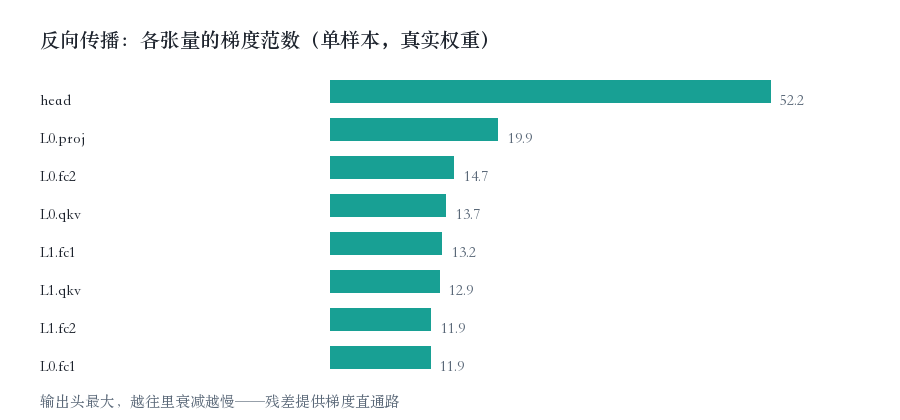
\includegraphics[width=0.8\linewidth]{../out/fig_grad.png}
\caption{反向传播中各张量的梯度范数（真实权重、单样本）。输出头最大，越往里衰减越慢
——残差提供了梯度直通路。}
\end{figure}

\section{从教学模型到控制器}

本教程的模型与项目里部署的控制器是同一个结构。把它变成控制器的全部差别只有三处：

\begin{enumerate}[leftmargin=1.6em,itemsep=3pt]
  \item \textbf{输入特征}：$F=6$，即 $[\sin\theta,\cos\theta,\dot\theta/4,\dot p/4,p/2.4,u_{k-1}/12]$，
        全部归一化到 $[-2,2]$；
  \item \textbf{窗口}：$T=24$（$0.48$\,s @ 50\,Hz），覆盖约 $1/3$ 个摆动周期；
  \item \textbf{输出限幅}：$u=12\tanh(\cdot)$，天然落在执行器的 $\pm12$\,N 内。
\end{enumerate}

部署时把它量化到 int8（$71$\,KB $\to$ $16.6$\,KB），单点最大误差 $0.14$\,N；
浏览器里手写前向（LayerNorm $\to$ 多头因果注意力 $\to$ GELU $\to\tanh$）单步 $0.32$\,ms。
手写前向之所以敢用，正是因为本教程这套"逐层对齐"的验证方法。

\section{习题}

\begin{enumerate}[leftmargin=1.6em,itemsep=6pt]
  \item 证明：若 $q,k$ 的各分量独立且方差为 $1$，则 $\mathrm{Var}(q^\top k)=d_h$。
        若方差为 $\sigma^2$ 呢？缩放因子应改成什么？
  \item 从 $\partial a_i/\partial s_j=a_i(\delta_{ij}-a_j)$ 出发，推导
        $\partial\mathcal{L}/\partial s_j=a_j(g_j-\sum_i a_ig_i)$。
  \item 把式 \eqref{eq:lnback} 展开成 $\partial\mu,\partial\sigma^2$ 两步，验证与紧凑式等价。
  \item 去掉残差（把 $z\leftarrow z+f(z)$ 改成 $z\leftarrow f(z)$），重跑 \texttt{parity\_test.py}
        与训练，比较第 0 层梯度范数与收敛速度。
  \item 把掩码值从 $-10^9$ 改成 $-1$，看训练会发生什么，并解释原因。
  \item 用 \texttt{numpy\_from\_state()} 加载生产权重，把 $d_h$ 从 8 改成 4（保持参数量），
        重训一次，比较闭环成功率。
\end{enumerate}

\section*{代码索引}
\addcontentsline{toc}{section}{代码索引}
\begin{center}
\small
\begin{tabular}{@{}ll@{}}
\toprule
文件 & 作用 \\
\midrule
\texttt{tinytf\_numpy.py} & 纯 numpy 实现：前向 + 手写反向 + AdamW \\
\texttt{tinytf\_torch.py} & 等价的 torch 实现 + 权重互转 \\
\texttt{parity\_test.py} & 与 autograd/有限差分对齐（本教程的可信度基石）\\
\texttt{train\_demo.py} & 双实现同条件训练对比（损失曲线、耗时）\\
\texttt{load\_pretrained.py} & 加载生产权重：一致性、闭环、注意力 \\
\texttt{make\_figs.py} & 生成文中三张图 \\
\bottomrule
\end{tabular}
\end{center}

\end{document}
